\newpage
\section{Revisão Teórica}
\subsection{Rede $L$}\label{subsec:l}
A rede L é a mais simples das redes e é largamente utilizada por isso \cite{Couch}. A rede L pode ser Passa-Baixas ou Passa-Altas, porém como neste trabalho o intuito da rede L é bloquear componentes DC, trabalharemos com a rede L Passa-Altas.

\begin{figure}[H]
    \centering
    \caption{Rede L passa-altas.}
    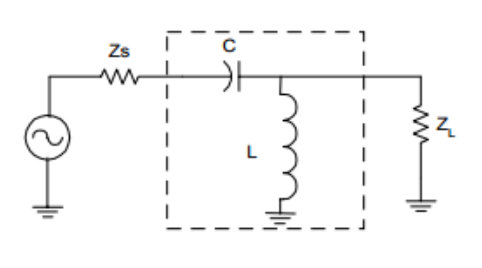
\includegraphics[scale=0.3]{Imagens/fig1.png}
    \label{f_fig1}
    
    \small Fonte: Taufik Abrão, 2002.
\end{figure}

Para o projeto de uma rede L, é necessário determinar seu valores de capacitância e indutância \cite{abrao, taufik1}. As equações (\ref{equ:ql}), (\ref{equ:xsl}) e (\ref{equ:xpl}) modelam a rede L. 

\begin{equation}
Q = \sqrt{\frac{R_L}{R_S}-1}.
\label{equ:ql}
\end{equation}

Onde Q é o fator de qualidade da rede, $R_S$ a resistência da fonte e $R_L$ a resistência da carga.

\begin{equation}
X_s = QR_S \ [\Omega].
\label{equ:xsl}
\end{equation}

Sendo $X_s$ a reatância do elemento série.

\begin{equation}
X_p = QR_L \ [\Omega].
\label{equ:xpl}
\end{equation}

Sendo $X_p$ a reatância do elemento em paralelo.

O valor dos componentes é determinado com os seguintes passos:

\begin{enumerate}
    \item cálculo do fator de qualidade Q de acordo com a impedância da fonte e da carga, conforme a equação (\ref{equ:ql});
    
    \item cálculo da reatância do elemento em série através da relação (\ref{equ:xsl});
        
    \item cálculo da reatância do elemento em paralelo através da relação (\ref{equ:xpl});
    
    \item determinação do valor dos componentes através do valor da reatância e da frequência de corte.
\end{enumerate}

\begin{figure}[H]
    \centering
    \caption{Parâmetros da rede L.}
    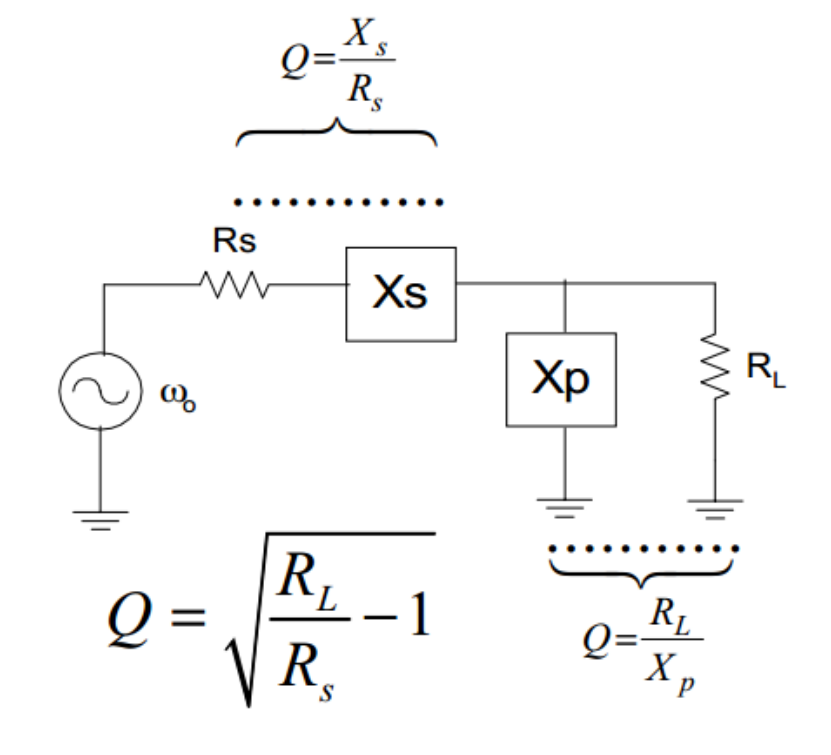
\includegraphics[scale=0.3]{Imagens/fig2.png}
    \label{f_fig2}
    
    \small Fonte: Taufik Abrão, 2002.
\end{figure}

Fator de qualidade em redes L está definido (fixo) pela relação entre $R_L$ e $R_S$ . Não há liberdade de escolha para o índice de qualidade o que é um dos grandes problemas no projeto de redes de banda estreita. Para resolver este problema, surgem as redes de três elementos que permitem obter adaptação de Z de banda estreita com alto Q.

\subsection{Rede $L_{wideband}$}\label{subsec:lwb}

Uma vez que em uma rede L, definido $R_S$ e $R_L$, fica determinado o índice de qualidade carregado da rede. Para adaptação de Z em circuitos de Banda Larga, usa-se duas (ou mais) Redes L em cascata (ou série). Para esse tipo de rede adaptadora, a resistência virtual $R_v$ está sempre entre os valores das resistências de fonte e carga. O índice de qualidade desse tipo de rede é menor que os de uma rede L simples, rede T ou rede $\pi$ . O valor de Q \cite{abrao} é dado por :

\begin{equation}
Q = \sqrt{\frac{R_v}{R_{min}} -1 }.
\label{equ:qlwb}
\end{equation}

Onde Q é o fator de qualidade carregado ($Q^{Load}$), $R_v$ é uma resistência virtual e $R_{min}$ é $min(R_L, R_S)$.

A máxima banda de passagem (ou mínimo Q) é obtida quando:

\begin{equation}
R_v = \sqrt{R_SR_L}.
\end{equation}

Conforme a necessidade de BW seja maior, mais redes L devem ser cascateadas.
As etapas de projeto para redes WBand de n seções L são as mesmas que as para uma rede L simples, basta solucionar a equação para um específico Q carregado baixo de projeto, obtendo $R_v$ e determinar a reatância dos elementos série e paralelo, porém, com as equações (\ref{equ:xs1}), (\ref{equ:xp1}), (\ref{equ:xs2}) e (\ref{equ:xp2}).

\begin{figure}[H]
    \centering
    \caption{Parâmetros da rede $L_{wideband}$.}
    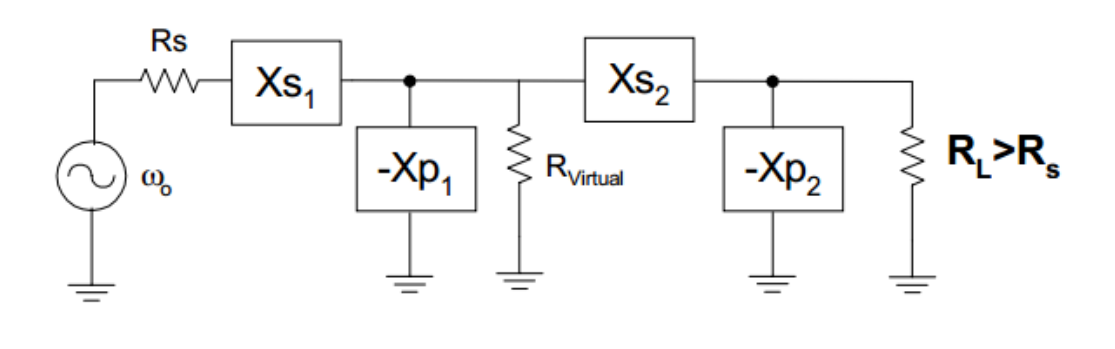
\includegraphics[scale=0.3]{Imagens/fig3.png}
    \label{f_fig3}
    
    \small Fonte: Taufik Abrão, 2002.
\end{figure}


\begin{equation}
X_{s1} = Q.
\label{equ:xs1}
\end{equation}

\begin{equation}
X_{p1} = Q.
\label{equ:xp1}
\end{equation}

\begin{equation}
X_{s2} = Q.
\label{equ:xs2}
\end{equation}

\begin{equation}
X_{p2} = Q.
\label{equ:xp2}
\end{equation}

\subsection{Rede $\pi$}\label{subsec:pi}

A rede $\pi$ consiste em duas redes L configuradas como "\textit{back to back}" \cite{abrao} onde o casamento de impedâncias é realizado através de um resistor virtual $R_v$, como mostra a figura \ref{fig:pi}.

\begin{figure}[H]
    \centering
    \caption{Parâmetros da rede $\pi$.}
    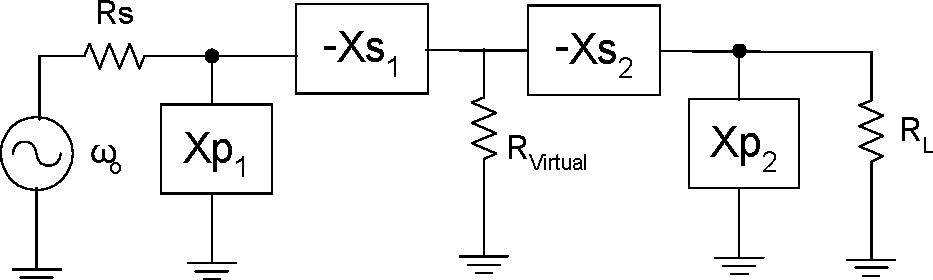
\includegraphics[scale=0.8]{Imagens/pi.pdf}
    \label{fig:pi}
    
    \small Fonte: Taufik Abrão, 2002.
\end{figure}

O processo para projeto da rede é semelhante ao da rede L, contudo, o fator Q é determinado de acordo com a equação (\ref{equ:qpi}).

\begin{equation}
Q = \sqrt{\frac{R_{high}}{R_{v}} -1 }.
\label{equ:qpi}
\end{equation}

Onde $R_{high} = max(R_S, \ R_L)$.

\subsection{Rede T}\label{subsec:t}

O projeto da rede T segue as mesmas etapas do projeto de uma rede $\pi$. Neste tipo de rede,
também deve-se adaptar a impedância da fonte à da carga via $R_{v}$ . A resistência virtual
na rede T é \cite{abrao, taufik1}: $R_v \ge  max(R_S, \ R_L)$.

\begin{figure}[H]
    \centering
    \caption{Parâmetros da rede $T$.}
    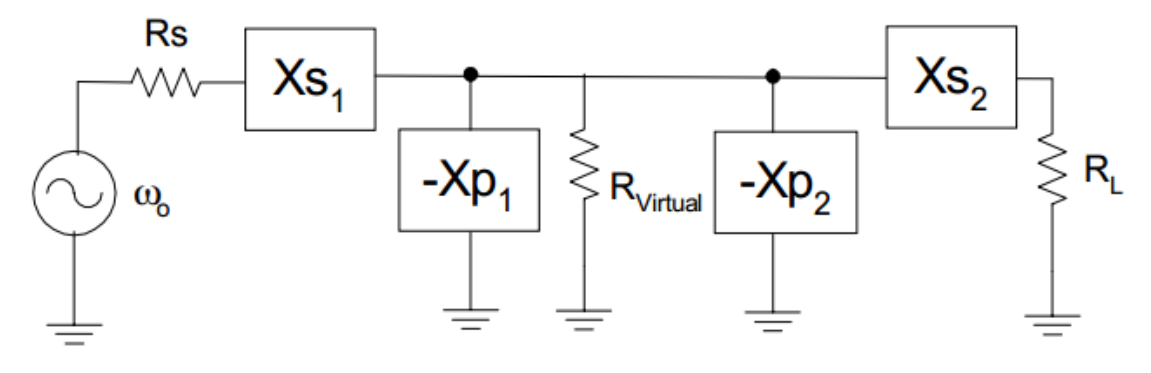
\includegraphics[scale=0.3]{Imagens/fig4.png}
    \label{f_fig4}
    
    \small Fonte: Taufik Abrão, 2002.
\end{figure}


Este tipo de rede é utilizada para adaptar duas impedâncias de baixo valor associado à necessidade de acoplamento em banda estreita (alto Q).
Q carregado da rede T é determinado pela seção L de maior Q (isto ocorre na terminação da seção L que tiver o menor resistor série de terminação), isto é $R_{Small} = min(R_S, \ R_L)$, conforme a equação (\ref{equ:qt}).

\begin{equation}
Q = \sqrt{\frac{R_v}{R_{small}} -1 }.
\label{equ:qt}
\end{equation}